\documentclass[11pt]{article}

\usepackage[margin=1in]{geometry}
\usepackage[T1]{fontenc}
\usepackage[utf8]{inputenc}
\usepackage{lmodern}
\usepackage{microtype}
\usepackage{amsmath,amssymb,mathtools}
\usepackage{booktabs}
\usepackage{enumitem}
\usepackage{xcolor}
\usepackage{tikz}
\usepackage{hyperref}
\usetikzlibrary{arrows.meta,positioning,fit,calc,shapes.geometric}

\hypersetup{
  colorlinks=true,
  linkcolor=blue!55!black,
  citecolor=blue!55!black,
  urlcolor=blue!55!black,
  pdftitle={Beneath the Skin: System and Mathematical Design},
  pdfauthor={Zhiyun Peng, Michael Tao, Eugene Fiume}
}

\definecolor{panelblue}{HTML}{0EA5E9}
\definecolor{panelgreen}{HTML}{22C55E}
\definecolor{panelamber}{HTML}{F59E0B}
\definecolor{panelbg}{HTML}{F8FAFC}
\definecolor{ink}{HTML}{0F172A}

\newcommand{\code}[1]{\texttt{#1}}
\newcommand{\R}{\mathbb{R}}
\newcommand{\clamp}{\operatorname{clamp}}

\title{\textbf{Beneath the Skin}\\System Architecture and Deformation Mathematics}
\author{Zhiyun Peng \and Michael Tao \and Eugene Fiume}
\date{Version 1.0 System Note}

\begin{document}
\maketitle

\begin{abstract}
This document describes the implemented system architecture and mathematical model for \emph{Beneath the Skin}, an interactive facial deformation dashboard for inspecting pose-driven blendshape activation, material transfer, and deformation telemetry.  The document is Overleaf-ready: it uses a self-contained LaTeX preamble, embeds diagrams with TikZ, and requires no external build tooling or generated figures.
\end{abstract}

\tableofcontents
\newpage

\section{System Overview}

\emph{Beneath the Skin} is a Vite application written in React and TypeScript.  The user-facing application starts at \code{src/main.tsx}, mounts \code{App}, and immediately enters \code{DashboardLayout}.  The dashboard composes five persistent regions:
\begin{enumerate}[leftmargin=*]
  \item the project hero, which identifies the research dashboard and selected provider;
  \item the Three.js viewport, which loads the glTF face mesh, textures, hair layer, tongue layer, and deformation runtime;
  \item the control panel, which emits preset, keyboard, slider, precompute, and optional projection-alignment commands;
  \item the live numeric readout, which displays current pose, frame, mode, and blendshape activations;
  \item the deformation curve panel, which samples activation energy over time using uPlot.
\end{enumerate}
The footer exposes citation and credit text for the project.

\begin{figure}[ht]
\centering
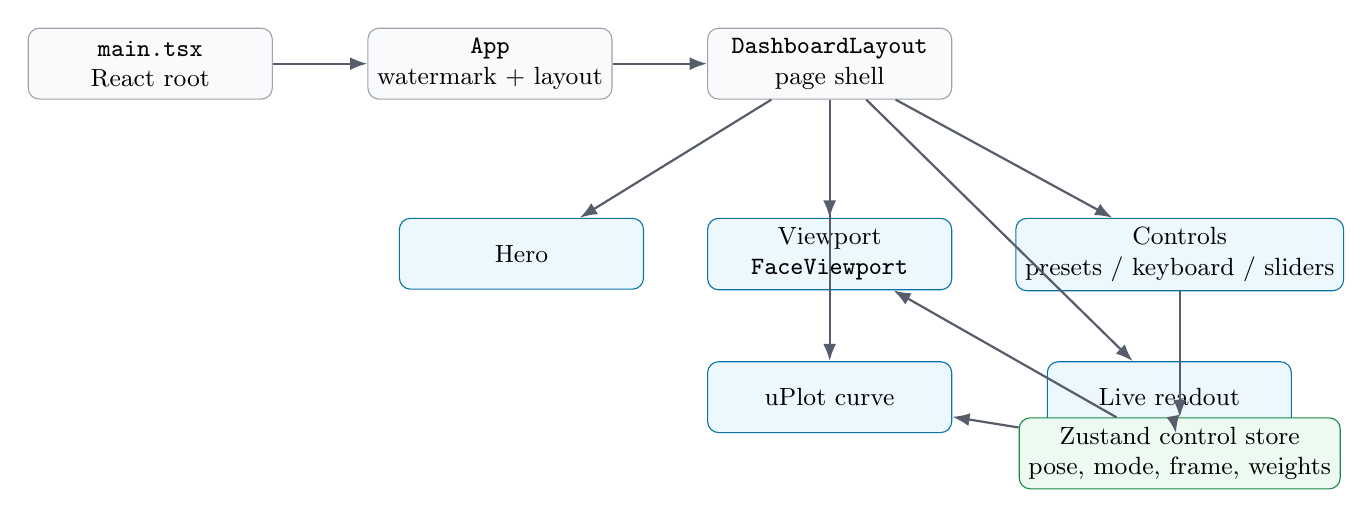
\begin{tikzpicture}[
  node distance=9mm and 12mm,
  box/.style={draw=ink!40, rounded corners, fill=panelbg, align=center, minimum width=31mm, minimum height=9mm, font=\small},
  region/.style={draw=panelblue!70!black, rounded corners, fill=panelblue!8, align=center, minimum width=31mm, minimum height=9mm, font=\small},
  state/.style={draw=panelgreen!70!black, rounded corners, fill=panelgreen!8, align=center, minimum width=34mm, minimum height=9mm, font=\small},
  arrow/.style={-{Latex[length=2.2mm]}, thick, draw=ink!70}
]
\node[box] (main) {\code{main.tsx}\\React root};
\node[box, right=of main] (app) {\code{App}\\watermark + layout};
\node[box, right=of app] (layout) {\code{DashboardLayout}\\page shell};

\node[region, below left=15mm and 8mm of layout] (hero) {Hero};
\node[region, below=15mm of layout] (viewport) {Viewport\\\code{FaceViewport}};
\node[region, below right=15mm and 8mm of layout] (controls) {Controls\\presets / keyboard / sliders};
\node[region, below=of viewport] (curve) {uPlot curve};
\node[region, right=of curve] (readout) {Live readout};
\node[state, below=16mm of controls] (store) {Zustand control store\\pose, mode, frame, weights};

\draw[arrow] (main) -- (app);
\draw[arrow] (app) -- (layout);
\draw[arrow] (layout) -- (hero);
\draw[arrow] (layout) -- (viewport);
\draw[arrow] (layout) -- (controls);
\draw[arrow] (layout) -- (curve);
\draw[arrow] (layout) -- (readout);
\draw[arrow] (controls) -- (store);
\draw[arrow] (store) -- (viewport);
\draw[arrow] (store) -- (curve);
\draw[arrow] (store) -- (readout);
\end{tikzpicture}
\caption{Entry flow and dashboard composition.  Controls write normalized state to Zustand; viewport, readout, and curve panels consume that state without duplicating control logic.}
\label{fig:entry-flow}
\end{figure}

\section{Technology Stack and Responsibilities}

\begin{table}[ht]
\centering
\begin{tabular}{@{}p{0.23\linewidth}p{0.67\linewidth}@{}}
\toprule
Layer & Responsibility \\
\midrule
React & Declares the dashboard regions, control surfaces, overlays, and lifecycle hooks for asset loading and frame updates. \\
TypeScript & Defines shared types for poses, provider frames, texture configuration, runtime diagnostics, and normalized control state. \\
Vite & Provides the browser build, static asset serving, environment-variable injection, and development server on port 8080. \\
Three.js & Owns glTF loading, materials, textures, geometry, morph-target influence arrays, lights, cameras, and procedural meshes. \\
react-three-fiber & Bridges React components to Three.js objects and supplies the per-frame \code{useFrame} loop used by the deformation runtime. \\
Zustand & Stores the canonical UI state: active pose label, active control mode, current frame index, and sparse activation weights. \\
uPlot & Renders the activation-energy time series in the deformation curve panel. \\
\bottomrule
\end{tabular}
\caption{Implemented stack responsibilities.}
\label{tab:stack}
\end{table}

The architecture deliberately keeps pose selection separate from deformation evaluation.  Controls never mutate Three.js morph-target arrays directly.  They emit normalized pose state.  The viewport runtime reads that state, asks the selected provider for a frame, and applies the resulting blendshape weights to the loaded mesh.

\section{Deformation Provider Abstraction}

The provider abstraction is defined by the \code{DeformationProvider} interface.  A provider exposes an identifier, a label, an initialization hook, a per-frame evaluator, an optional precompute hook, and an optional disposal hook.  The runtime-visible frame shape is common across provider implementations:
\begin{itemize}[leftmargin=*]
  \item \code{blendshapeWeights}: the sparse, normalized blendshape influence map used by the current implementation;
  \item \code{vertexDeltas}: an optional extension point for providers that produce direct vertex or normal deltas;
  \item \code{frameIndex} and \code{progress}: telemetry for readout and animation state.
\end{itemize}

The registry in \code{src/domain/providers/provider-registry.ts} is the extension point.  The current default entry is \code{kinematic-blendshape}; the environment loader validates \code{VITE\_DEFORMATION\_PROVIDER} against the registry before the app boots.  A future precomputed provider or biomechanical simulation provider would add a registry entry and return the same \code{DeformationFrame} contract.  The controls, readout, and curve panels would remain unchanged because they depend on target poses and runtime frames, not on provider internals.

\begin{figure}[ht]
\centering
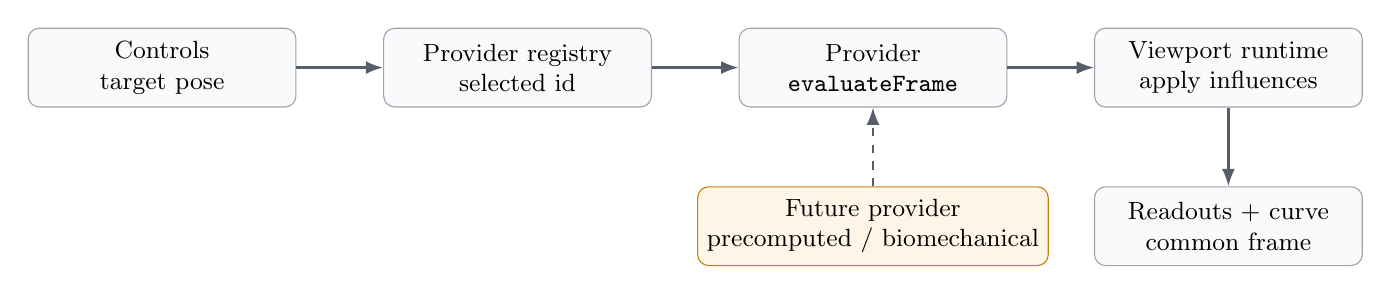
\begin{tikzpicture}[
  node distance=10mm and 11mm,
  box/.style={draw=ink!40, rounded corners, fill=panelbg, align=center, minimum width=34mm, minimum height=10mm, font=\small},
  ext/.style={draw=panelamber!80!black, rounded corners, fill=panelamber!10, align=center, minimum width=37mm, minimum height=10mm, font=\small},
  arrow/.style={-{Latex[length=2.2mm]}, thick, draw=ink!70}
]
\node[box] (controls) {Controls\\target pose};
\node[box, right=of controls] (registry) {Provider registry\\selected id};
\node[box, right=of registry] (provider) {Provider\\\code{evaluateFrame}};
\node[box, right=of provider] (runtime) {Viewport runtime\\apply influences};
\node[box, below=of runtime] (readouts) {Readouts + curve\\common frame};
\node[ext, below=of provider] (future) {Future provider\\precomputed / biomechanical};

\draw[arrow] (controls) -- (registry);
\draw[arrow] (registry) -- (provider);
\draw[arrow] (provider) -- (runtime);
\draw[arrow] (runtime) -- (readouts);
\draw[arrow, dashed] (future) -- (provider);
\end{tikzpicture}
\caption{Provider boundary.  New deformation algorithms slot behind the registry and preserve the UI-facing frame contract.}
\label{fig:provider-boundary}
\end{figure}

\section{Blendshape Deformation Mathematics}

Let the neutral face mesh contain $n$ vertices.  Stack the neutral vertex positions into
\begin{equation}
  \mathbf{x}_0 \in \R^{3n}.
\end{equation}
For each exposed morph target $j$, let
\begin{equation}
  \Delta \mathbf{x}_j = \mathbf{x}_j - \mathbf{x}_0
\end{equation}
be the morph-target displacement from neutral.  A posed face is modeled as a weighted linear blend:
\begin{equation}
  \mathbf{x}(\mathbf{w}) = \mathbf{x}_0 + \sum_{j \in \mathcal{M}} w_j \Delta \mathbf{x}_j,
  \label{eq:blendshape-linear}
\end{equation}
where $\mathcal{M}$ is the set of morph targets exposed by the loaded mesh and each influence $w_j$ is clamped to the unit interval:
\begin{equation}
  w_j = \clamp(\hat{w}_j, 0, 1).
\end{equation}

Pose definitions are authored as sparse maps from semantic blendshape names to target weights.  At provider initialization, the loaded mesh reports its morph-target dictionary.  The resolver first tries exact names, then generated and curated aliases such as ARKit-style camel case, snake case, side suffixes, and project-specific fallbacks.  If no exposed target resolves for a requested name, that entry is filtered out of the runtime blend and surfaced in diagnostics as missing rather than silently pretending to deform.

For a transition from previous weights $\mathbf{a}$ to target weights $\mathbf{b}$, the runtime evaluates a smooth interpolation.  With normalized progress $p \in [0,1]$, the smoothstep blend factor is
\begin{equation}
  s(p) = p^2(3 - 2p),
\end{equation}
and each output influence is
\begin{equation}
  w_j(p) = \clamp\left(a_j + \left(b_j-a_j\right)s(p), 0, 1\right).
  \label{eq:smoothstep-weight}
\end{equation}
After interpolation, weights at or below the small activation epsilon are dropped from the sparse frame map.  This keeps neutral or near-neutral frames compact and avoids stale tiny activations appearing in the readout.

\section{Pose Library, Compatibility Audit, and Diagnostics}

The pose library groups entries into phonemes, expressions, and FACS action units.  Each entry stores a label, category, description, optional code or keyboard key, and provider-specific weight map.  The current set covers neutral, N, AA, IY, T, EH, UW, V, Y, the supported expressions, and the FACS action-unit sliders.

On mesh load and pose changes, the provider-health overlay runs a compatibility audit.  For each referenced blendshape in the active pose, the audit records:
\begin{description}[leftmargin=*]
  \item[active] the weight is above epsilon and resolves to a morph target exposed by the mesh;
  \item[missing] the weight is above epsilon but no morph target or alias resolves;
  \item[unsupported] the entry is effectively inactive after clamping, usually because its authored weight is zero.
\end{description}
The library summary counts neutral, supported, partial, and unsupported poses.  The overlay reports the active-pose counts plus aggregate library counts so an inert or partially supported pose is visible during testing.

\section{Transition Precompute Cache}

Keyboard mode can switch quickly between many pose pairs.  To avoid first-time evaluation lag during interactive use, pairwise keyboard-pose transitions can be precomputed.  The warmup set contains neutral plus all keyboard-mapped poses.  For each ordered pair $(P_i,P_k)$, the cache stores a fixed number of frames:
\begin{equation}
  F = 18.
\end{equation}
The cached frame for offset $r \in \{1,\ldots,F\}$ uses progress
\begin{equation}
  p_r = \frac{r}{F}
\end{equation}
and the same provider evaluation path as live frames.  The cache key includes provider id, source pose label, and target pose label.  At runtime, a cached frame is reused only when the current source weights are nearly equal to the cached source weights.  If the cache entry is missing or the source weights differ, the runtime evaluates the frame live.  This preserves correctness for slider mixes and other non-keyboard states while accelerating common keyboard transitions.

\section{Control Modes and State Flow}

The canonical UI state lives in the Zustand control store.  It contains the active pose label, active mode, current frame index, and sparse activation map.  All state writes pass through normalization:
\begin{equation}
  \operatorname{normalize}(v)_j =
  \begin{cases}
    \clamp(v_j,0,1), & \text{if } j \text{ is nonempty and } \clamp(v_j,0,1)>\epsilon,\\
    \varnothing, & \text{otherwise.}
  \end{cases}
\end{equation}
The implementation uses $\epsilon=0.001$ for UI activation storage.

\subsection{Preset Mode}
Preset dropdowns select a phoneme, expression, or action unit.  The selected pose is resolved for the configured provider and written to the store with mode \code{preset}, frame index zero, and the pose's normalized activation map.

\subsection{Keyboard Mode}
Keyboard mode is enabled explicitly.  Keyboard handlers ignore modified keys, repeated keys, and editable elements.  Valid keys map to pose entries, then use the same pose application path as preset mode but write mode \code{keyboard}.  Switching into or out of keyboard mode resets state to neutral so previous animations do not leak into the new mode.

\subsection{Slider Mode}
The muscle slider panel exposes FACS action-unit controls.  A slider value $\alpha_i \in [0,1]$ scales each basis pose's blendshape weights.  If $b_{ij}$ is blendshape $j$'s authored basis weight in slider $i$, the composite slider activation is
\begin{equation}
  c_j = \clamp\left(\sum_i \alpha_i\,\clamp(b_{ij},0,1), 0, 1\right).
  \label{eq:slider-composition}
\end{equation}
Near-zero composites are dropped.  If at least one activation remains, the active pose label becomes \code{Slider Mix}; otherwise it returns to neutral.

\subsection{Preventing Stale Feedback}
The frame runtime writes evaluated weights back to the store so readouts and the curve reflect interpolated values, not just the final target.  To prevent stale animation feedback from overriding a user-selected mode, the store accepts runtime activation writes only when the write's mode matches the current active mode.  Mode changes reset frame index and activation values to neutral.

\section{Activation-Energy Metric}

The deformation curve panel samples the current activation map and computes a bounded root-mean-square energy:
\begin{equation}
  E(\mathbf{w}) =
  \begin{cases}
    0, & |\mathcal{A}|=0,\\
    \min\left(1,\sqrt{\dfrac{1}{|\mathcal{A}|}\sum_{j\in\mathcal{A}} w_j^2}\right), & |\mathcal{A}|>0,
  \end{cases}
  \label{eq:activation-energy}
\end{equation}
where $\mathcal{A}$ is the set of currently active blendshapes.  Samples are keyed by frame index.  If a new value arrives for the current frame, the existing sample is updated; otherwise a new sample is appended.  The panel retains a rolling window of at most 160 samples and plots energy in the range $[0,1]$ with uPlot.

\section{Texture and Material Handling}

The app supports three separate diffuse maps:
\begin{itemize}[leftmargin=*]
  \item \code{VITE\_SKIN\_TEXTURE\_URL}: skin/head/body atlas;
  \item \code{VITE\_EYE\_TEXTURE\_URL}: eye, iris, pupil, and sclera texture;
  \item \code{VITE\_ORAL\_TEXTURE\_URL}: teeth, gums, palate, oral cavity, and tongue texture.
\end{itemize}
Each defaults to a committed asset under \code{public/textures}.  Diffuse textures are loaded with sRGB color space and \code{flipY=false} to match glTF UV orientation.  Load failures resolve to \code{null}, emit a warning, and leave procedural material settings in place rather than breaking the viewport.

Material slots are classified by mesh and material names.  Eye and oral textures are direct-assignment only: the loader assigns them only to matching standard-material slots that expose UVs.  If those slots are absent or unsuitable, the app reports skipped slots and does not project the texture onto unrelated geometry.

\subsection{Direct Skin Assignment}
The direct skin path is used when skin material slots appear to match the supplied atlas layout.  A slot is considered a direct candidate when it is skin-intent, uses a standard material, has a UV attribute, and the mesh/material naming indicates a head, face, skin, body, neck, shoulder, chest, torso, or FaceCap-style slot.  Direct assignment provides highest fidelity because it uses artist-authored UVs.

\subsection{UV-Independent Projected Transfer}
When direct UV assignment is not reliable, the projected transfer path builds a replacement UV channel from world-space positions.  Let the loaded head's bounding box be
\begin{equation}
  B = [x_{\min},x_{\max}]\times[y_{\min},y_{\max}]\times[z_{\min},z_{\max}],
\end{equation}
with center $(x_c,y_c,z_c)$.  For a vertex position $\mathbf{q}=(x,y,z)$ transformed to world space, the projection first rotates the horizontal coordinates about the vertical axis by configurable angle $\theta$:
\begin{align}
  x' &= (x-x_c)\cos\theta - (z-z_c)\sin\theta.
\end{align}
Then it computes atlas coordinates
\begin{align}
  u_0 &= \frac{x'}{\max(x_{\max}-x_{\min},\,z_{\max}-z_{\min})}+\frac{1}{2},\\
  v_0 &= 1 - \frac{y-y_{\min}}{y_{\max}-y_{\min}}.
\end{align}
Projection alignment applies scale $\sigma$ and offsets $(o_u,o_v)$ around the center:
\begin{align}
  u &= \clamp((u_0-1/2)\sigma + 1/2 + o_u,0,1),\\
  v &= \clamp((v_0-1/2)\sigma + 1/2 + o_v,0,1).
\end{align}
The generated UVs are attached to a cloned geometry, preserving morph targets and blendshape influence arrays.  The texture map is then assigned to the same standard material, so normal lighting, roughness, and metalness behavior remain material-driven.

\begin{figure}[ht]
\centering
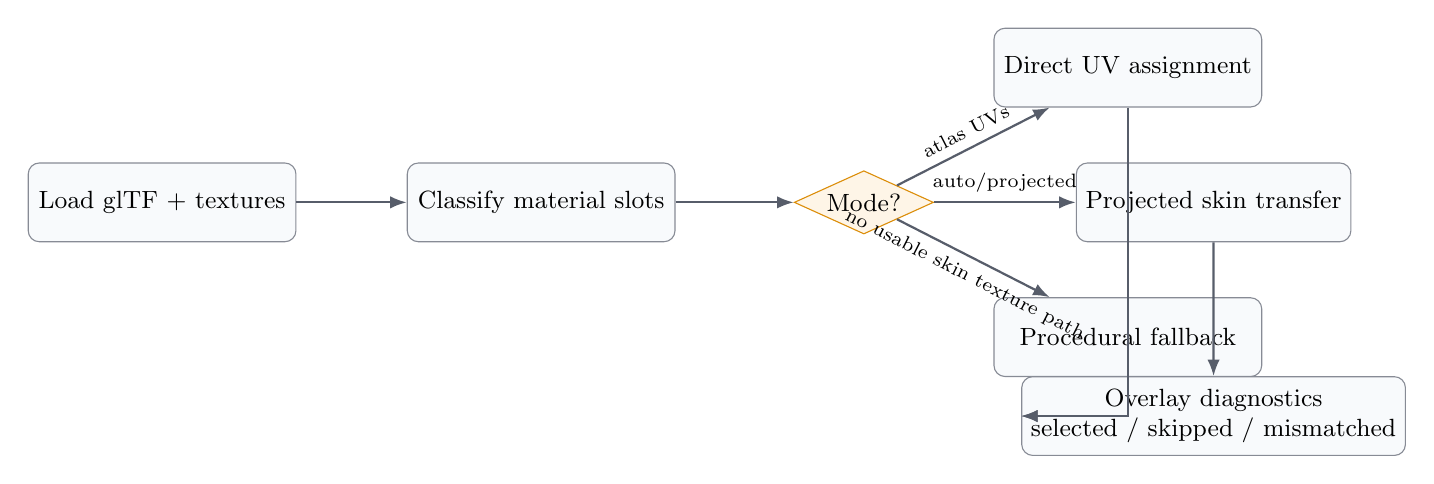
\begin{tikzpicture}[
  scale=0.95,
  box/.style={draw=ink!50, rounded corners, fill=panelbg, align=center, minimum width=34mm, minimum height=10mm, font=\small},
  decision/.style={diamond, draw=panelamber!90!black, fill=panelamber!10, aspect=2.2, align=center, inner sep=1.5pt, font=\small},
  arrow/.style={-{Latex[length=2.1mm]}, thick, draw=ink!70}
]
\node[box] (load) {Load glTF + textures};
\node[box, right=14mm of load] (slots) {Classify material slots};
\node[decision, right=15mm of slots] (mode) {Mode?};
\node[box, above right=10mm and 12mm of mode] (uv) {Direct UV assignment};
\node[box, right=18mm of mode] (proj) {Projected skin transfer};
\node[box, below right=10mm and 12mm of mode] (proc) {Procedural fallback};
\node[box, below=17mm of proj] (diag) {Overlay diagnostics\\selected / skipped / mismatched};

\draw[arrow] (load) -- (slots);
\draw[arrow] (slots) -- (mode);
\draw[arrow] (mode) -- node[above, sloped, font=\scriptsize]{atlas UVs} (uv);
\draw[arrow] (mode) -- node[above, font=\scriptsize]{auto/projected} (proj);
\draw[arrow] (mode) -- node[below, sloped, font=\scriptsize]{no usable skin texture path} (proc);
\draw[arrow] (uv) |- (diag);
\draw[arrow] (proj) -- (diag);
\draw[arrow] (proc) |- (diag);
\end{tikzpicture}
\caption{Texture-transfer selection and diagnostics.  Eye and oral textures bypass projected transfer and use direct UV slots only.}
\label{fig:texture-transfer}
\end{figure}

\subsection{Mode Selection and Accuracy Trade-offs}
The configured transfer mode is \code{auto}, \code{projected}, or \code{uv}.  In \code{auto}, the loader selects direct UV assignment when all skin slots are direct candidates; otherwise it prefers projected transfer for eligible standard-material skin meshes.  Explicit \code{uv} or \code{projected} requests are honored when their required slots exist.  If neither path is usable, the system leaves the procedural material in place and reports the mismatch.

Projected transfer is robust to unknown UV layouts and makes the committed atlas visible on arbitrary head meshes, but it is approximate.  Because it derives atlas coordinates from a bounding box, local features such as brows, lip edges, and eye openings can drift relative to the mesh topology.  The projection-alignment panel exposes horizontal offset, vertical offset, scale, and vertical-axis rotation behind the same feature-flag pattern as optional panels.  These controls allow interactive registration tuning, but they do not replace the fidelity of offline texture baking or mesh-specific UV authoring.

\section{Hair, Tongue, and Oral Integration}

Hair is optional.  If \code{VITE\_HAIR\_MESH\_URL} is configured, the viewport loads a separate glTF hair mesh, normalizes it to the head, and applies dark rough material settings.  If no asset is configured or the load fails, a procedural dark hair cap is rendered.  Hair is a separate scene object and does not touch the face mesh's morph targets.

Tongue rendering is tied to oral texture support and phoneme activation.  During head loading, material and morph-target names are inspected for tongue geometry or tongue-related morph targets.  When a loaded mesh already provides tongue geometry, the system leaves that geometry under the mesh's own morph-target deformation.  When no tongue geometry is detected, the viewport adds a small procedural tongue mesh inside the mouth cavity.  It samples the tongue region of the oral atlas when available, falls back to a procedural pink material if the oral texture fails, and remains hidden except when a tongue activation is present.  The T phoneme includes a strong \code{tongueOut} target with complementary mouth and jaw weights so tongue movement reads as part of the articulation.

\section{Runtime Diagnostics}

The viewport overlays combine asset status, provider health, texture transfer, hair status, and tongue status.  The diagnostics are intentionally visible in the shipped dashboard because the same UI is used both as a demo and as a regression inspection surface.  The provider-health panel reports active blendshape compatibility, missing and unsupported targets, library-level support counts, selected texture transfer mode, projection alignment values, and skipped or mismatched material slots.

\section{Conclusion}

The implemented system separates control intent, provider evaluation, mesh application, and telemetry.  This separation keeps the current kinematic blendshape provider simple while leaving a clear route for future precomputed or biomechanical deformation providers.  The material-transfer layer similarly offers a direct high-fidelity path, a robust projected path, and explicit diagnostics for mesh mismatches.

\begin{thebibliography}{9}

\bibitem{facs}
Paul Ekman and Wallace V. Friesen.
\newblock \emph{Facial Action Coding System: A Technique for the Measurement of Facial Movement}.
\newblock Consulting Psychologists Press, 1978.

\bibitem{beneath-skin}
Zhiyun Peng, Michael Tao, and Eugene Fiume.
\newblock \emph{Beneath the Skin}.
\newblock Research project paper, formal publication metadata pending.

\bibitem{threejs}
Three.js contributors.
\newblock \emph{Three.js Documentation}.
\newblock \url{https://threejs.org/docs/}.

\bibitem{react-three-fiber}
pmndrs contributors.
\newblock \emph{react-three-fiber Documentation}.
\newblock \url{https://docs.pmnd.rs/react-three-fiber/}.

\end{thebibliography}

\end{document}
